\documentclass[aspectratio=169,10pt]{beamer}

\usetheme{default}
\usefonttheme{professionalfonts}

\usepackage[T1]{fontenc}
\usepackage{lmodern}
\usepackage{amsmath,amssymb,bm}
\usepackage{booktabs}
\usepackage{graphicx}
\usepackage{mathtools}
\usepackage{xcolor}

\definecolor{MSEBlue}{RGB}{24,61,104}
\definecolor{MSEGray}{RGB}{92,101,116}
\definecolor{MSELight}{RGB}{245,247,250}
\definecolor{MSEGreen}{RGB}{0,115,88}
\definecolor{MSERed}{RGB}{170,50,50}

\setbeamertemplate{navigation symbols}{}
\setbeamertemplate{footline}{
  \leavevmode%
  \hbox{%
  \begin{beamercolorbox}[wd=.72\paperwidth,ht=2.7ex,dp=1.1ex,leftskip=1.8em]{author in head/foot}%
    \scriptsize Sequential Tradeability Testing for Alpha Signals
  \end{beamercolorbox}%
  \begin{beamercolorbox}[wd=.28\paperwidth,ht=2.7ex,dp=1.1ex,rightskip=1.8em plus 1fil]{date in head/foot}%
    \hfill \scriptsize \insertframenumber/\inserttotalframenumber
  \end{beamercolorbox}}%
}
\setbeamertemplate{itemize item}{\raisebox{0.15ex}{\scriptsize$\blacktriangleright$}}
\setbeamertemplate{itemize subitem}{\scriptsize$\circ$}
\setbeamertemplate{blocks}[rounded][shadow=false]

\setbeamercolor{title}{fg=MSEBlue}
\setbeamercolor{frametitle}{fg=MSEBlue}
\setbeamercolor{normal text}{fg=black,bg=white}
\setbeamercolor{structure}{fg=MSEBlue}
\setbeamercolor{block title}{fg=white,bg=MSEBlue}
\setbeamercolor{block body}{fg=black,bg=MSELight}
\setbeamerfont{frametitle}{size=\Large,series=\bfseries}
\setbeamerfont{title}{size=\LARGE,series=\bfseries}
\setbeamerfont{subtitle}{size=\large}

\newcommand{\E}{\mathbb{E}}
\newcommand{\Var}{\operatorname{Var}}
\newcommand{\F}{\mathcal{F}}
\newcommand{\dd}{\,d}
\newcommand{\wh}{\widehat}
\newcommand{\wt}{\widetilde}
\newcommand{\Lgen}{\mathcal{L}}
\newcommand{\1}{\mathbf{1}}

\title{Sequential Tradeability Testing for Alpha Signals}
\subtitle{A Bayesian optimal stopping view of alpha validation}
\author{Rany Stephan}
\institute{MSE342 Project}
\date{\today}

\begin{document}

\begin{frame}
  \titlepage
  \vspace{-0.7em}
  \begin{center}
    \color{MSEGray}
    \large When should a we stop researching a signal and admit it to live trading?
  \end{center}
\end{frame}

\begin{frame}{Portfolio optimization needs trusted alpha}
  \large
  \[
  \begin{aligned}
    \max_{w}\quad &
      \alpha^\top w
      \;-\;\frac{\gamma}{2}\,w^\top\Sigma\,w
      \;-\;\mathrm{Cost}(w-w_0)\\[2pt]
    \text{s.t.}\quad
      & \mathbf 1^\top w = 1,
      \qquad \ell \le w \le u,\\[1pt]
      & F^\top w = f,
      \qquad \|w-w_0\|_1 \le \tau .
  \end{aligned}
  \]

  \vspace{0.2em}
  \footnotesize
  \(w\) weights, \(w_0\) current holdings, \(\Sigma=F\Sigma_f F^\top+D\) factor risk,
  \(\mathrm{Cost}(\cdot)\) spread \(+\) impact, \(F\) factor loadings, \(\tau\) turnover budget.
  \normalsize

  \vspace{0.5em}
  Risk, constraints, and trading costs can be modeled carefully.
  \textbf{But what admits \(\alpha\)?}

  \vspace{0.4em}
  \begin{block}{The upstream question}
    \(\alpha\) is not a given input: it is an uncertain object learned from noisy evidence,
    and the most fragile input in the pipeline. This project is the \emph{alpha-validation
    layer}: which signals have enough evidence to be admitted as \(\alpha\). It is not a
    replacement for the optimizer.
  \end{block}
\end{frame}

\begin{frame}{The object of the project}
  \begin{center}
  \large
  research evidence arrives over time
  \(\quad\Longrightarrow\quad\)
  continue, activate, or reject
  \end{center}

  \vspace{1.0em}

  \begin{block}{Thesis}
    Alpha validation is a stopping problem under posterior uncertainty: evidence
    acquisition has option value, while delay, decay, and implementation costs enter the
    payoff.
  \end{block}

  \vspace{0.8em}
  \normalsize
  EKV supplies a tractable posterior diffusion. The project replaces squared-error
  terminal loss with an economic admission payoff.
\end{frame}

\begin{frame}{Fixed horizons are not admission rules}
  \begin{columns}[T,onlytextwidth]
    \begin{column}{0.48\textwidth}
      \begin{block}{Fixed-horizon test}
        \[
          \text{at } T:\quad \text{is the signal significant?}
        \]
        \begin{itemize}
          \item conditions on an exogenous date;
          \item separates statistical evidence from implementation value;
          \item delays both activation and rejection.
        \end{itemize}
      \end{block}
    \end{column}
    \begin{column}{0.48\textwidth}
      \begin{block}{Sequential admission}
        \[
          \tau:\quad \text{continue, activate, or reject}
        \]
        \begin{itemize}
          \item endogenous decision time;
          \item stopping region partitions activation and rejection;
          \item continuation prices one more observation.
        \end{itemize}
      \end{block}
    \end{column}
  \end{columns}
\end{frame}

\begin{frame}{Storyline}
  \large
  \begin{enumerate}
    \item EKV: learn an unknown drift from noisy Brownian evidence.
    \item Key identity: posterior uncertainty is also the speed of learning.
    \item Project move: replace EKV's terminal statistical loss with an economic alpha payoff.
    \item Stress test: Gaussian beliefs capture learning option value but rule out a point-mass null.
    \item Extension: a three-state prior makes the null-alpha state explicit.
    \item Evidence: OSAP and WRDS experiments compare sequential admission with fixed horizons.
  \end{enumerate}
\end{frame}

\section{The EKV foundation}

\begin{frame}{EKV starts with drift learning}
  \Large
  \[
    Y_t = X\,t + W_t,\qquad t\ge 0 .
  \]

  \vspace{0.8em}

  \normalsize
  \begin{itemize}
    \item \(X\) is an unknown constant drift drawn from a prior \(\mu\).
    \item \(Y_t\) is cumulative noisy evidence.
    \item \(\F_t^Y=\sigma(Y_s:0\le s\le t)\) is the information available to the decision maker.
  \end{itemize}

  \vspace{0.6em}
  \begin{block}{Alpha interpretation}
    For signal validation, \(X\) is latent alpha strength (the signal's risk-adjusted
    excess-return edge) and \(Y_t\) is normalized cumulative return evidence.
  \end{block}
\end{frame}

\begin{frame}{Bayes' rule gives the posterior state}
  \Large
  \[
    \mu_{t,y}(du)
    =
    \frac{\exp\{uy-u^2t/2\}\mu(du)}
    {\int_{\mathbb R}\exp\{vy-v^2t/2\}\mu(dv)} .
  \]

  \vspace{0.8em}

  \begin{columns}[T,onlytextwidth]
    \begin{column}{0.48\textwidth}
      \[
        \wh X_t = G(t,Y_t)
      \]
      \[
        G(t,y)=\E[X\mid Y_t=y]
      \]
    \end{column}
    \begin{column}{0.48\textwidth}
      \[
        H(t,y)=\Var(X\mid Y_t=y)
      \]
      \[
        \partial_y G(t,y)=H(t,y)
      \]
    \end{column}
  \end{columns}

  \vspace{0.4em}
  \normalsize
  The posterior mean and posterior variance are the low-dimensional state variables.
\end{frame}

\begin{frame}{The filtering identity}
  \Large
  \[
    \wt W_t
    =
    Y_t-\int_0^t\wh X_s\,ds
    \quad\text{(innovation, a } \F^Y\text{-Brownian motion)}
  \]

  \vspace{0.4em}

  \[
    d\wh X_t=\Psi(t,\wh X_t)\,d\wt W_t,
    \qquad
    \Psi(t,\wh X_t)=\Var(X\mid \F_t^Y).
  \]

  \vspace{0.6em}
  \begin{block}{Intuition}
    The posterior mean is an \(\F_t^Y\)-martingale. The single quantity \(\Psi\) is both the
    remaining estimation error and the local volatility of belief revisions: the state
    variable and the learning rate at once.
  \end{block}
\end{frame}

\begin{frame}{EKV's optimal stopping problem}
  \Large
  \[
    \inf_\tau
    \E\left[(X-\wh X_\tau)^2+c\tau\right].
  \]

  \vspace{0.7em}

  \normalsize
  EKV study the optimal time to stop observing and report the posterior mean.

  \pause
  \vspace{1.0em}
  \Large
  \[
    \E[\Psi(\tau,\wh X_\tau)]
    =
    \Var(X)
    -
    \E\!\left[\int_0^\tau \Psi^2(s,\wh X_s)\dd s\right].
  \]

  \vspace{0.4em}
  \footnotesize
  (Posterior variance \(=\) mean-squared error; Itô on the martingale \(\wh X\) gives
  quadratic variation \(\Psi^2\).) Expected posterior variance decreases by accumulated
  squared learning speed.
\end{frame}

\begin{frame}{The EKV problem becomes a running-cost problem}
  \Large
  \[
    \inf_\tau
    \E\left[
      \int_0^\tau
      \left(c-\Psi^2(s,\wh X_s)\right)\dd s
    \right].
  \]

  \vspace{1.0em}

  \begin{columns}[T,onlytextwidth]
    \begin{column}{0.45\textwidth}
      \begin{block}{Cost of waiting}
        \[
          c
        \]
        observation and opportunity cost
      \end{block}
    \end{column}
    \begin{column}{0.45\textwidth}
      \begin{block}{Benefit of waiting}
        \[
          \Psi^2
        \]
        instantaneous variance reduction
      \end{block}
    \end{column}
  \end{columns}
\end{frame}

\begin{frame}{Two EKV benchmarks we use to validate the math}
  \begin{columns}[T,onlytextwidth]
    \begin{column}{0.48\textwidth}
      \begin{block}{Gaussian prior}
        \[
          X\sim N(m_0,q_0)
        \]
        \[
          q(t)=\frac{q_0}{1+q_0t},
          \qquad
          dm_t=q(t)\,d\wt W_t .
        \]
        \[
          \tau^\star=\left(\frac{1}{\sqrt c}-\frac{1}{q_0}\right)^+ .
        \]
      \end{block}
    \end{column}
    \begin{column}{0.48\textwidth}
      \begin{block}{Symmetric Bernoulli prior}
        \[
          X\in\{-\beta,\beta\},
          \qquad
          \Psi(x)=\beta^2-x^2 .
        \]
        Continuation is a symmetric band in posterior mean: the continuous-time
        sequential probability ratio test geometry.
      \end{block}
    \end{column}
  \end{columns}
\end{frame}

\section{Our alpha admission problem}

\begin{frame}{The project changes the terminal reward}
  \large
  \[
    \text{EKV: estimate accurately}
    \qquad
    \Longrightarrow
    \qquad
    \text{finance: admission payoff}
  \]

  \vspace{1.0em}

  \normalsize
  \begin{block}{Scope of transfer}
    EKV gives the posterior state process. The finance boundary is obtained by changing
    the reward functional and solving the induced obstacle problem.
  \end{block}
\end{frame}

\begin{frame}{Variable translation}
  \large
  \begin{center}
  \begin{tabular}{lll}
    \toprule
    EKV object & & Alpha validation object \\
    \midrule
    \(X\) & & unknown alpha strength \\
    \(Y_t\) & & cumulative normalized evidence \\
    \(\wh X_t\) & & posterior mean alpha \\
    \(\Psi\) & & posterior uncertainty and learning speed \\
    \(c\) & & research cost, delay, opportunity cost \\
    \(\tau\) & & activation or rejection time \\
    \bottomrule
  \end{tabular}
  \end{center}
\end{frame}

\begin{frame}{Economic activation payoff}
  \Large
  \[
    mz-\frac{\lambda}{2}(\sigma_r^2+q)z^2-\kappa .
  \]

  \vspace{0.5em}
  \footnotesize
  \(m=\wh X\) posterior mean alpha, \(q=\Psi\) posterior parameter risk, \(z\) exposure,
  \(\lambda\) risk aversion, \(\sigma_r^2\) return variance, \(\kappa\) implementation hurdle.
  \normalsize

  \pause
  \vspace{0.3em}
  The objective is concave in \(z\); the optimum and optimized value are closed form:

  \vspace{0.3em}
  \Large
  \[
    z^\star=\frac{m}{\lambda(\sigma_r^2+q)},
    \qquad
    \Phi(m,q)
    =
    \left(
      \frac{m^2}{2\lambda(\sigma_r^2+q)}
      -\kappa
    \right)^+ .
  \]

  \pause
  \vspace{0.4em}
  \normalsize
  \[
    |m|>\sqrt{2\lambda(\sigma_r^2+q)\kappa}
  \]
  is the static activation threshold. The stopping boundary also incorporates the option
  value of future evidence.
\end{frame}

\begin{frame}{The finite-horizon stopping problem}
  \Large
  \[
    V(t,m)
    =
    \sup_{\tau\in[t,T]}
    \E_{t,m}\left[
      e^{-\rho\tau}\Phi(m_\tau,q(\tau))
      -
      \int_t^\tau c\,ds
    \right].
  \]

  \vspace{0.7em}

  \pause
  \normalsize
  With obstacle \(g(t,m)=e^{-\rho t}\Phi(m,q(t))\) and generator
  \(\Lgen_t V=\tfrac12 q(t)^2 V_{mm}\), the value solves the variational inequality

  \vspace{0.3em}
  \Large
  \[
    \max\left\{
      \,g-V,\;
      V_t+\Lgen_t V-c
    \right\}=0,
    \qquad V\ge g .
  \]

  \pause
  \vspace{0.2em}
  \normalsize
  Continuation region \(\mathcal C=\{V>g\}\), stopping region \(\mathcal S=\{V=g\}\),
  separated by a free boundary with value matching \(V=g\) (smooth pasting where regular).

  \vspace{0.3em}
  \footnotesize
  \emph{Convention:} discounting sits in the time-dependent obstacle \(e^{-\rho t}\Phi\)
  (calendar-time value), so no \(-\rho V\) term; equivalently \(e^{-\rho(\tau-t)}\) would
  move it into the continuation operator.
\end{frame}

\begin{frame}{What the boundary means}
  \begin{columns}[T,onlytextwidth]
    \begin{column}{0.56\textwidth}
      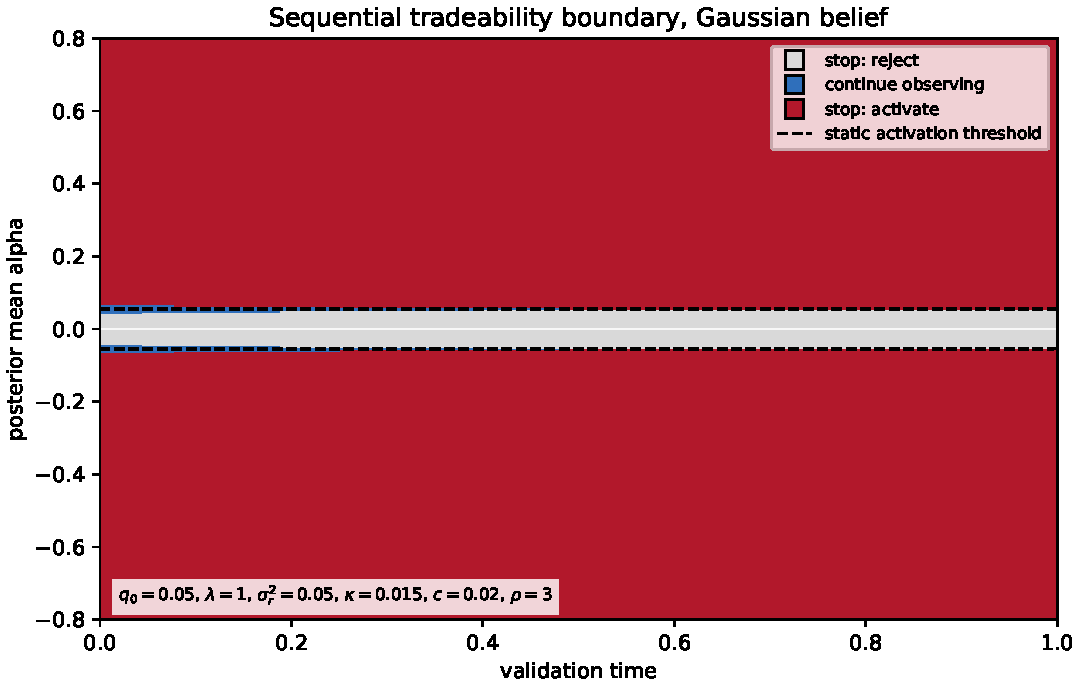
\includegraphics[width=\linewidth]{../figures/gaussian_tradeability_boundary.pdf}
    \end{column}
    \begin{column}{0.40\textwidth}
      \begin{itemize}
        \item Red: stop and activate \((\mathcal S)\).
        \item Gray: stop and reject \((\mathcal S)\).
        \item Blue: continue observing \((\mathcal C)\).
        \item Dashed: static activation threshold.
        \item Lines: two posterior-mean paths.
      \end{itemize}
      \vspace{0.5em}
      The continuation region \(\mathcal C\) is a value-of-information region, not a
      positive-payoff region.
    \end{column}
  \end{columns}
\end{frame}

\begin{frame}{First stress test: Gaussian beliefs}
  \begin{columns}[T,onlytextwidth]
    \begin{column}{0.58\textwidth}
      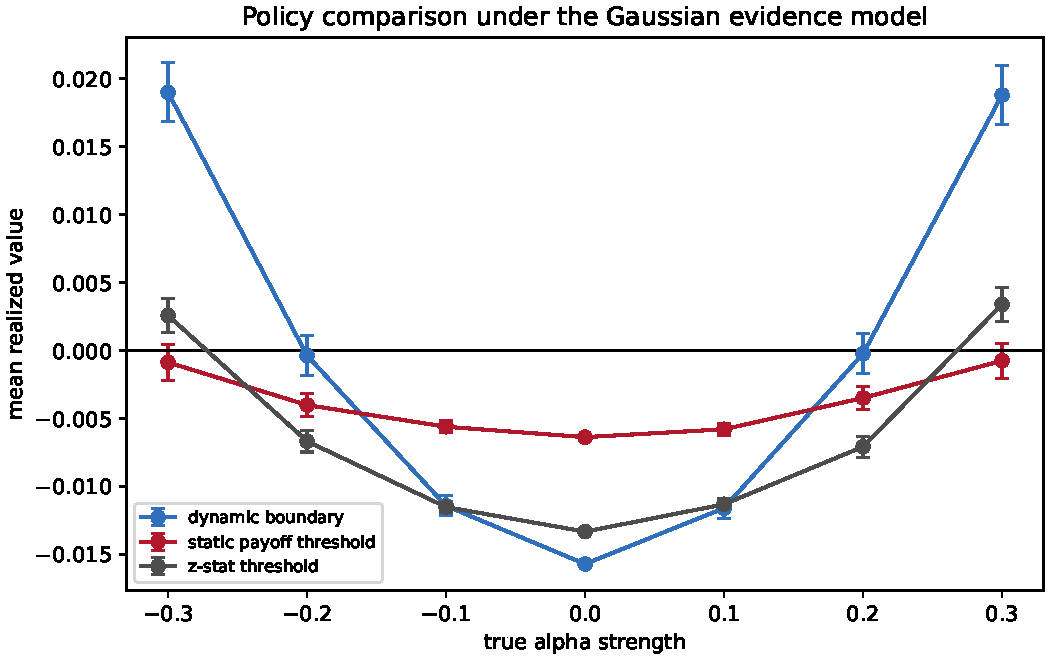
\includegraphics[width=\linewidth]{../figures/simulation_policy_comparison.pdf}
    \end{column}
    \begin{column}{0.38\textwidth}
      \begin{block}{Model success}
        For large \(|\theta|\), dynamic stopping extracts learning option value.
      \end{block}
      \begin{block}{Model limitation}
        At \(\theta=0\), the Gaussian prior activates about \(90.1\%\) of null paths.
      \end{block}
    \end{column}
  \end{columns}
\end{frame}

\begin{frame}{The Gaussian prior rules out a point-mass null}
  \Large
  \[
    X\sim N(0,q_0)
    \quad \Rightarrow \quad
    \mathbb P(X=0)=0 .
  \]

  \vspace{1.0em}
  \normalsize
  A diffuse Gaussian prior treats the null as an event of posterior probability zero.
  That is a structural mismatch when the candidate set may contain signals with no
  admissible economic alpha.

  \vspace{0.8em}
  \begin{block}{Implication}
    Introduce an explicit null-alpha state and let posterior evidence move mass into or
    out of that state.
  \end{block}
\end{frame}

\section{Three-state alpha prior}

\begin{frame}{A three-state prior for alpha admission}
  \Large
  \[
    \theta\in\{-a,0,+a\}.
  \]

  \vspace{0.8em}

  \begin{center}
  \begin{tabular}{cl}
    \toprule
    State & Interpretation \\
    \midrule
    \(-a\) & negative alpha \\
    \(0\) & null alpha \\
    \(+a\) & positive alpha \\
    \bottomrule
  \end{tabular}
  \end{center}

  \vspace{0.8em}
  \normalsize
  The state space now separates sign uncertainty from the probability of no admissible
  alpha.
\end{frame}

\begin{frame}{Posterior probabilities under the three-state prior}
  \Large
  \[
    \pi_i(t,y)
    =
    \frac{
      p_i\exp\{\theta_i y-\theta_i^2t/2\}
    }{
      \sum_j p_j\exp\{\theta_j y-\theta_j^2t/2\}
    } .
  \]

  \vspace{0.7em}
  \[
    m(t,y)=\sum_i\pi_i(t,y)\theta_i,
    \qquad
    q(t,y)=\sum_i\pi_i(t,y)\theta_i^2-m(t,y)^2 .
  \]

  \vspace{0.5em}
  \normalsize
  Near-zero cumulative evidence increases the posterior mass on \(\theta=0\), because
  nonzero drift states are less consistent with a persistent absence of direction.
\end{frame}

\begin{frame}{False-discovery penalty}
  \Large
  \[
    \Phi_\eta(t,y)
    =
    e^{-\rho t}
    \left(
      \frac{m(t,y)^2}{2\lambda(\sigma_r^2+q(t,y))}
      -\kappa-\eta\pi_0(t,y)
    \right)^+ .
  \]

  \vspace{0.8em}
  \normalsize
  The term \(\eta\pi_0(t,y)\) is the posterior expected cost of admitting a null-alpha
  signal.

  \pause
  \vspace{0.5em}
  \Large
  \[
    \max\left\{
      \Phi_\eta-V,\,
      V_t+\Lgen_t V-c
    \right\}=0,
    \quad
    \Lgen_t f=m(t,y)f_y+\tfrac12 f_{yy} .
  \]

  \vspace{0.2em}
  \footnotesize
  With three states the posterior mean is no longer a sufficient coordinate, so the value
  is solved in \emph{evidence space} \(y\). There \(\Lgen_t\) is the generator of the
  posterior-predictive evidence \(dY_t=m(t,Y_t)\,dt+d\wt W_t\); solved by a monotone upwind
  scheme.
\end{frame}

\begin{frame}{Controlled validation of the three-state rule}
  \begin{columns}[T,onlytextwidth]
    \begin{column}{0.58\textwidth}
      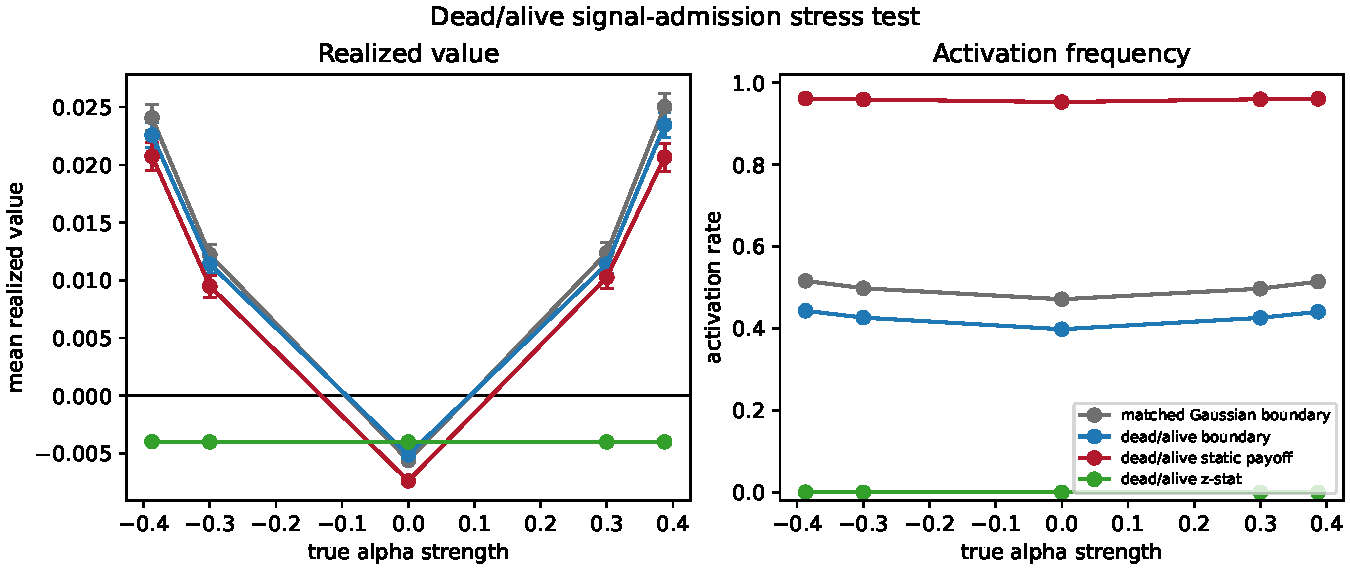
\includegraphics[width=\linewidth]{../figures/dead_alive_policy_comparison.pdf}
    \end{column}
    \begin{column}{0.38\textwidth}
      \begin{block}{Null activation}
        \[
          47.1\% \to 39.8\%
        \]
        matched Gaussian boundary versus three-state boundary.
      \end{block}
      \begin{block}{Null realized value}
        \[
          -0.00560 \to -0.00513
        \]
      \end{block}
      The rule trades lower null activation against slightly lower live-alpha value.
    \end{column}
  \end{columns}
\end{frame}

\section{Real data}

\begin{frame}{Real-data design}
  \large
  \begin{center}
  \begin{tabular}{ll}
    \toprule
    Data & Chen-Zimmermann Open-Source Asset Pricing (OSAP) long-short returns \\
    Eligible signals & 192 predictors with enough history \\
    Calibration & 120 months \\
    Sequential validation & up to 240 months \\
    Holdout & 120 post-decision months \\
    Evidence increment & \(\Delta Y_t=(r_t/\widehat\sigma_m)\sqrt{dt}\) \\
    Placebo & sign-flipped validation returns \\
    \bottomrule
  \end{tabular}
  \end{center}

  \vspace{0.6em}
  \normalsize
  Under a null with monthly variance \(\widehat\sigma_m^2\),
  \(\Var(\Delta Y_t)\approx dt\), so evidence is on Brownian scale.
\end{frame}

\begin{frame}{Penalty calibration with real signals and placebos}
  \begin{columns}[T,onlytextwidth]
    \begin{column}{0.58\textwidth}
      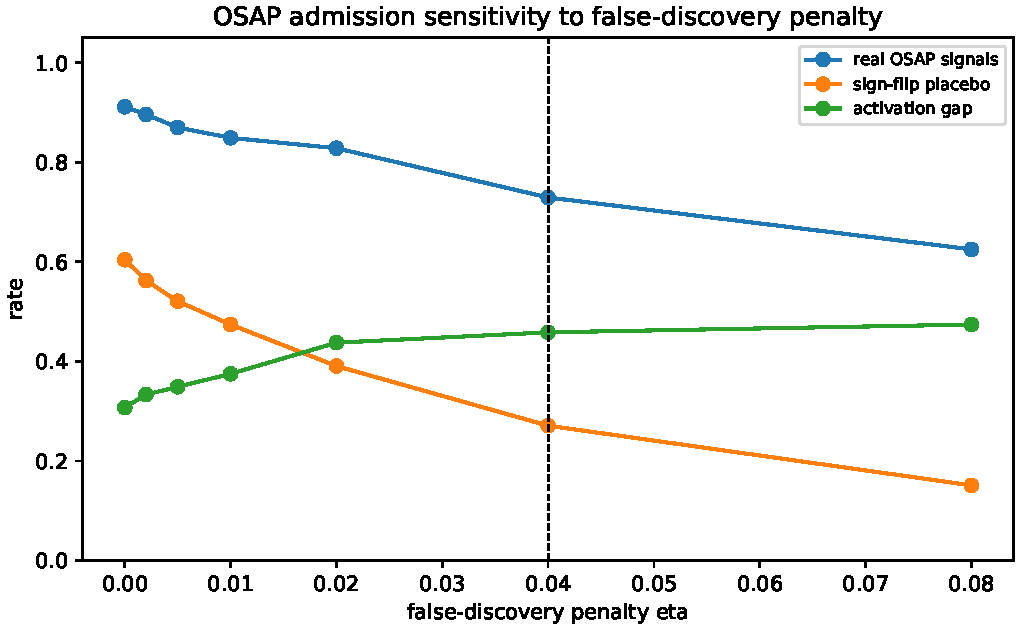
\includegraphics[width=\linewidth]{../figures/osap_penalty_sweep.pdf}
    \end{column}
    \begin{column}{0.38\textwidth}
      \begin{block}{At \(\eta=0.04\)}
        \[
          \text{real activation}=72.9\%
        \]
        \[
          \text{placebo activation}=27.1\%
        \]
      \end{block}
      The placebo activation rate is more sensitive to the penalty than the real-signal
      activation rate.
    \end{column}
  \end{columns}
\end{frame}

\begin{frame}{Is the rule really sequential?}
  \begin{columns}[T,onlytextwidth]
    \begin{column}{0.58\textwidth}
      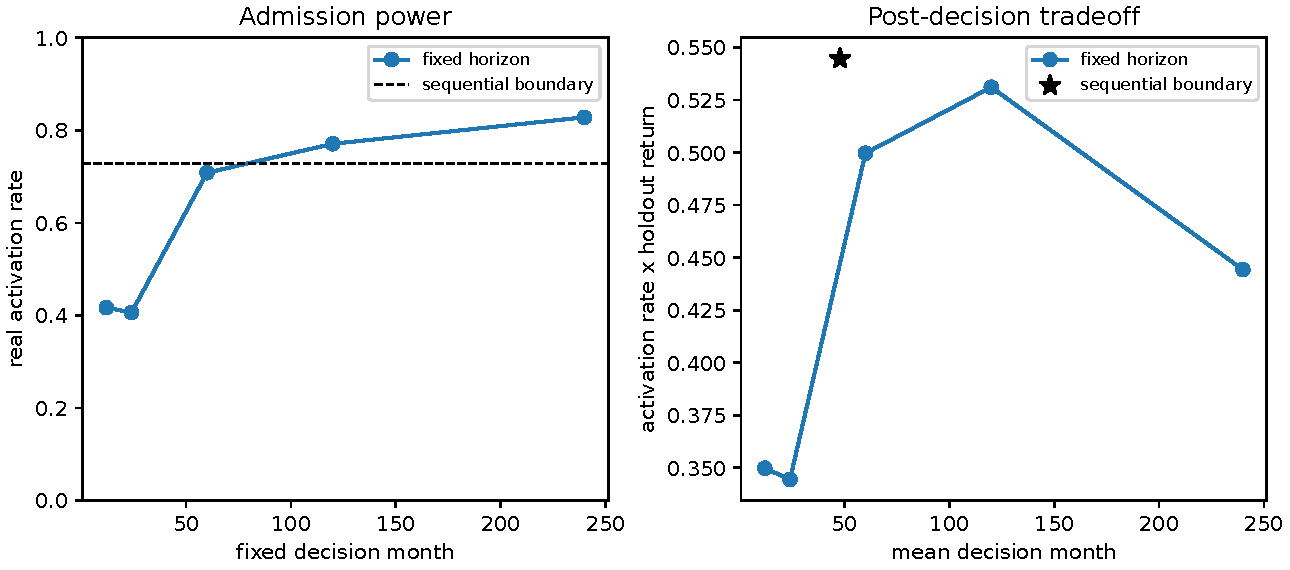
\includegraphics[width=\linewidth]{../figures/osap_static_benchmark_comparison.pdf}
    \end{column}
    \begin{column}{0.38\textwidth}
      \pause
      \begin{block}{Sequential rule}
        \[
          72.9\% \text{ real activation}
        \]
        \[
          47.9 \text{ month average decision time}
        \]
        \[
          0.545 \text{ activation-weighted holdout}
        \]
      \end{block}
      \pause
      Longer fixed horizons increase admission power, but at substantially later decision
      dates and lower activation-weighted holdout returns.
    \end{column}
  \end{columns}
\end{frame}

\begin{frame}{WRDS stock-level reconstruction}
  \large
  \begin{center}
  \begin{tabular}{lrrrr}
    \toprule
    Return stream & \(N\) & Active & Standard active & Std. holdout \\
    \midrule
    Gross stock-level & 3 & 3 & 3 & \(1.227\%\) \\
    Net range-cost stress & 3 & 3 & 0 & n/a \\
    \bottomrule
  \end{tabular}
  \end{center}

  \vspace{0.6em}
  \footnotesize
  Three signals rebuilt from CRSP/Compustat via WRDS (Wharton Research Data Services).
  \normalsize
  Gross long-short returns are admitted in the standard direction. The range-cost proxy
  (turnover \(\times\) monthly high-low range) removes several percent per month, turning
  posterior net drift negative: the symmetric rule would then activate by \emph{shorting},
  so standard-direction admissions are zero.

  \vspace{0.3em}
  The experiment separates statistical signal evidence from implementable signal value.
\end{frame}

\section{Checks and conclusion}

\begin{frame}{Mathematical and numerical checks}
  \large
  \begin{itemize}
    \item Posterior probabilities remain positive and sum to one.
    \item \(\partial_y G(t,y)=H(t,y)\) and \(\partial_y m(t,y)=q(t,y)\) are checked numerically.
    \item Gaussian posterior precision update matches the closed form.
    \item The obstacle solver satisfies terminal value, symmetry, and monotonicity tests.
    \item Dead/alive finite-difference diagnostics: zero obstacle violation, zero terminal error,
      symmetry error \(4.2\times10^{-16}\).
    \item Grid convergence: the paper grid has \(V(0,0)\) error below \(9\times10^{-5}\)
      relative to the fine grid.
  \end{itemize}
\end{frame}

\begin{frame}{What is novel here?}
  \large
  \begin{itemize}
    \item The EKV filtering state is used for alpha validation rather than drift estimation alone.
    \item The terminal payoff is economic: posterior alpha must clear risk, uncertainty, and costs.
    \item The three-state prior makes the null-alpha probability part of the state.
    \item The empirical test asks whether sequential stopping beats fixed-horizon posterior tests
      at matched placebo activation.
  \end{itemize}

  \vspace{0.8em}
  \begin{block}{One-line conclusion}
    Alpha validation is a sequential admission problem, not a fixed-date significance test.
  \end{block}
\end{frame}

\begin{frame}{Final takeaways}
  \Large
  \begin{enumerate}
    \item EKV gives a rigorous Bayesian learning state.
    \item Economic tradeability changes the stopping reward.
    \item Gaussian beliefs reveal the learning option value but exclude a point-mass null.
    \item A three-state prior reduces null activation in simulation and placebo tests.
    \item Real data suggest earlier admission at comparable placebo-calibrated power.
  \end{enumerate}
\end{frame}

\begin{frame}{References}
  \small
  \begin{thebibliography}{9}
    \bibitem{ekv}
    Ekstrom, Karatzas, and Vaicenavicius.
    \newblock Bayesian Sequential Least-Squares Estimation for the Drift of a Wiener Process.
    \newblock \emph{Stochastic Processes and their Applications}, 2022.

    \bibitem{cz}
    Chen and Zimmermann.
    \newblock Open Source Cross-Sectional Asset Pricing.
    \newblock \emph{Critical Finance Review}, 2022.

    \bibitem{cv}
    Chen and Velikov.
    \newblock Zeroing In on the Expected Returns of Anomalies.
    \newblock \emph{Journal of Financial and Quantitative Analysis}, 2023.
  \end{thebibliography}
\end{frame}

\end{document}
